\documentclass{beamer}
%\usetheme{Boadilla}

\usepackage[utf8]{inputenc}
\usepackage[french]{babel} %pour la typographie française.
\usepackage[T1]{fontenc} %pour la césure des mots.
\usepackage{amssymb} %pour les symboles mathématiques et lettres grecques
\usepackage{amsmath} %pour les formules mathématiques avancées
\usepackage{listings} %lstlisting
\usepackage{xcolor} % pour mettre du texte en couleur
\usepackage{tikz}
\usetikzlibrary{calc, trees, positioning, arrows, shapes, shapes.multipart, shadows, matrix, decorations.pathreplacing, decorations.pathmorphing, automata}
\definecolor{vert}{RGB}{0,153,0}

\beamertemplatenavigationsymbolsempty % Option pour supprimer la barre de navigation dans les slides

\title{Projet TriComp : Présentation}
\author{Equipe TriComp}
\date{Jeudi 18 Décembre 2014}

% Faire apparaître un sommaire avant chaque section
\AtBeginSection[]{
   \begin{frame}{Plan}
%   \begin{center}{\Large Plan }\end{center}
   %%% affiche en début de chaque section, les noms de sections et
   %%% noms de sous-sections de la section en cours.
   \tableofcontents[currentsection]
   \end{frame}
}

\begin{document}

\frame{
   \begin{center}
        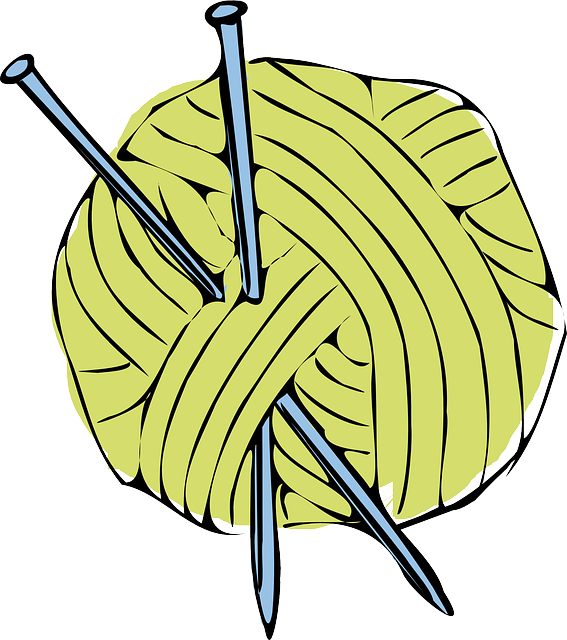
\includegraphics[height=0.2\textheight]{../img/ball_of_wool.png}
        \hspace*{4cm}
        
\includegraphics[height=0.2\textheight]{../img/logo_ens.jpg}
   \end{center}
   \titlepage
}

\frame{
	\frametitle{Plan}
		\tableofcontents
}

\section{Introduction}

\frame{
	\frametitle{L'équipe TriComp}
		\begin{center}
			{\large
			{William \textsc{Aufort} \hspace{4cm} Julien \textsc{Bensmail} \\}
			\vspace{1cm}
			{Agathe \textsc{Herrou}  \hspace{4cm} Romain \textsc{Labolle} \\}
			\vspace{1cm}
			{Frédéric \textsc{Lang} \hspace{4cm} Maxime \textsc{Lesourd} \\}
			\vspace{1cm}
			{Laureline \textsc{Pinault} \hspace{3.7cm} Léo \textsc{Stéfanesco} \\}}
		\end{center}
}

\subsection{Motivations}

\frame{

  \frametitle{Motivations}
  \begin{itemize}
    \onslide<2-> \item Tricot peu présent dans le milieu informatique
    \onslide<3-> \item Logiciels de tricot incomplets : pas d'instructions
    \onslide<4-> \item Représentation inefficace des tricots (matrices de points)
    % Deux raisons d'automatiser le calcul des instructions
    \onslide<5-> \item Des instructions longues, compliquées à établir, et qui ne tiennent pas compte de la forme du tricot dans les ouvrages.
    \onslide<6-> \item Un projet original !
  \end{itemize}
}

\subsection{Quelques notions de tricot}

\frame{
	\frametitle{Quelques notions de tricot...}
        \begin{columns}
          \column{0.6\textwidth}
          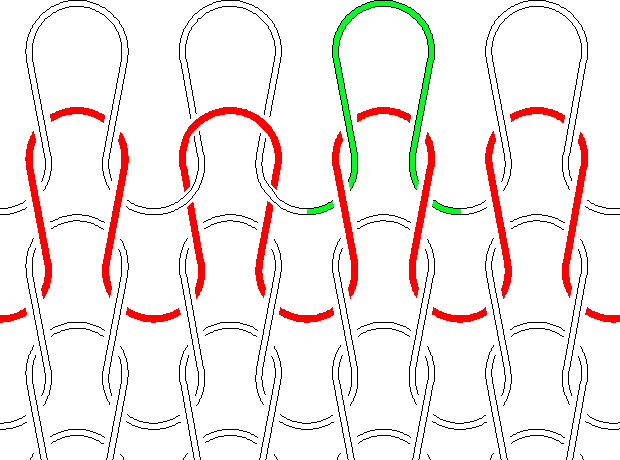
\includegraphics[scale=0.3]{Knit-schematic.png}
          \column{0.4\textwidth}
          \begin{itemize}
            \pause
          \item[] \textcolor{green}{maille}
            \pause
          \item[] \textcolor{red}{rang}
          \end{itemize}
        \end{columns}
}

\frame{
	\frametitle{Quelques notions de tricot...}
        \begin{columns}
          \column{0.6\textwidth}
          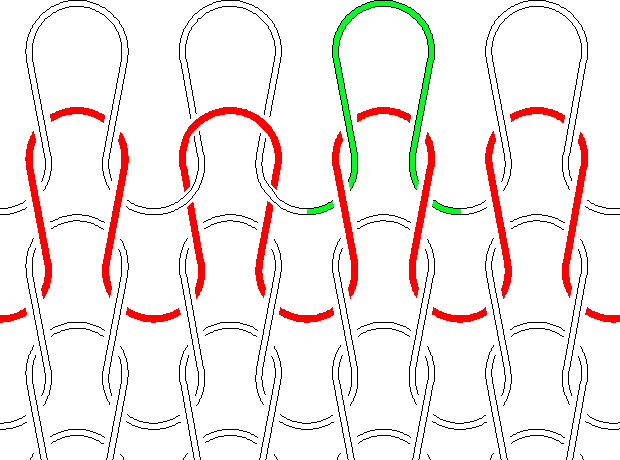
\includegraphics[scale=0.3]{Knit-schematic.png}
          \column{0.4\textwidth}
          \begin{itemize}
          \item[] \textcolor{green}{maille à l'endroit}
          \item[]
          \end{itemize}
        \end{columns}
}
\frame{
	\frametitle{Quelques notions de tricot...}
        \begin{columns}
          \column{0.6\textwidth}
          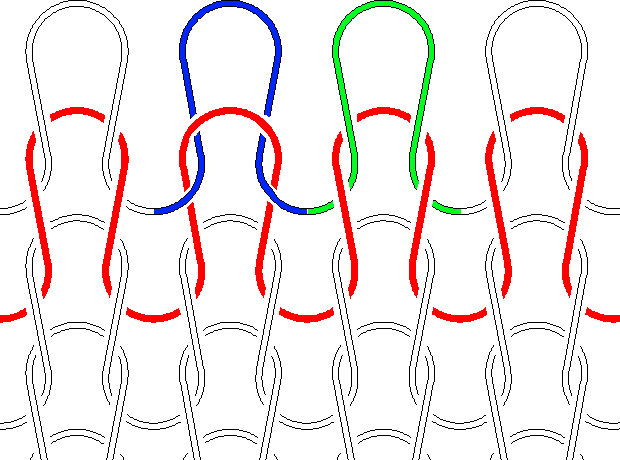
\includegraphics[scale=0.3]{Knit-schematic2.png}
          \column{0.4\textwidth}
          \begin{itemize}
          \item[] \textcolor{green}{maille à l'endroit}
          \item[] \textcolor{blue}{maille à l'envers}
          \end{itemize}
        \end{columns}
}

\frame{
  \frametitle{Rendu}
  \begin{center}
    \includegraphics[scale=0.08]{../img/Stockinette_example_front.JPG}
  \end{center}
}

\frame{
  \frametitle{Rendu}
  \begin{center}
    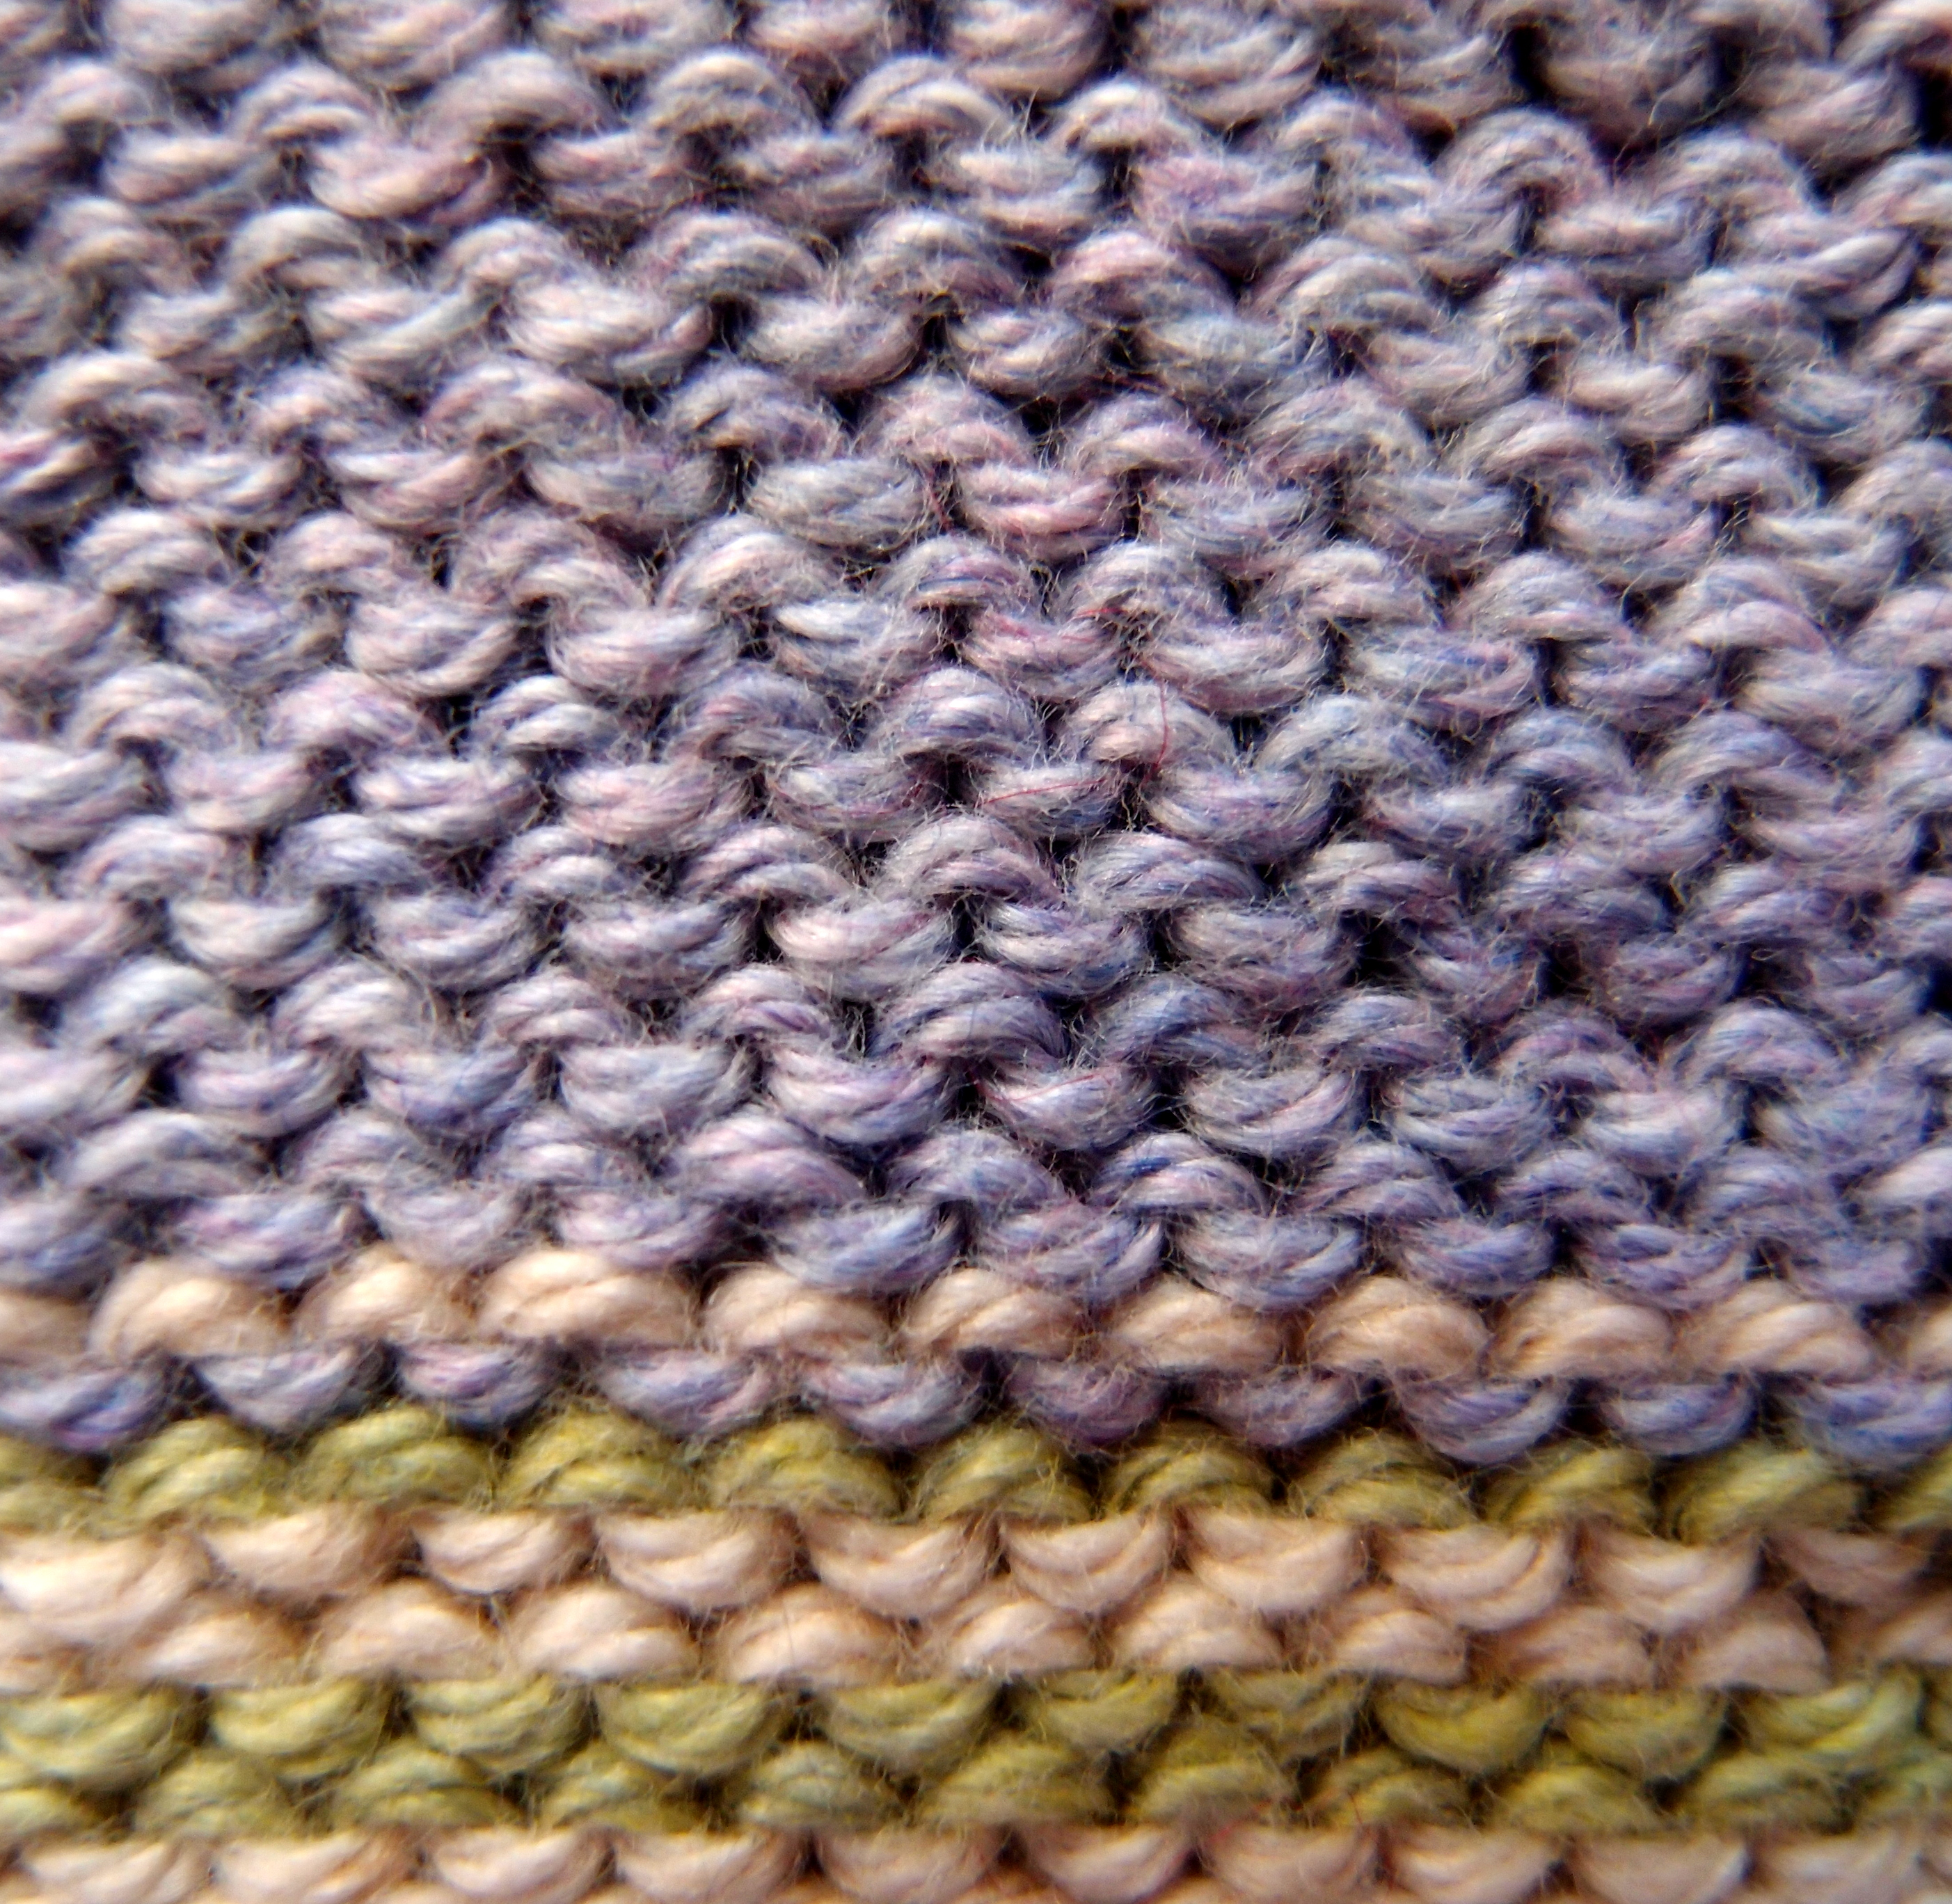
\includegraphics[scale=0.08]{../img/Stockinette_example_back.JPG}
  \end{center}
}

\frame{
	\frametitle{Les instructions de tricot}
			Les instructions à suivre par le tricoteur comportent des informations sur :
			\begin{itemize}
				\item le type de point à tricoter
				\item le nombre de points identiques
				\item le nombre de rangs à reproduire
			\end{itemize}
                        $\Rightarrow$ Description d'un motif minimal à répéter
			% TODO : Un exemple d'instructions de tricot
}

\subsection{Présentation générale}

\frame{
	\frametitle{TriComp : un compilateur pour tricot}
	\begin{figure}[!h]
		\centering
		\begin{tikzpicture}[->, >=stealth', shorten >=1pt, auto, node distance = 3.5cm, semithick]
			\tikzstyle{every state}=[draw=black,text=black,shape=rectangle]
		    \node[single arrow, draw, align=center, xshift=0cm, yshift=5cm, rotate=0, minimum height=4em](compilateur)[xshift=-1cm]
				{Compilateur};
%		    \node[state] (compilateur) [shape=arrow] 	{Compilateur};
		    \node[rectangle, draw, minimum height=10em, minimum width=7em, align=center](patron-d)[left of=compilateur,xshift=0.5cm]
				{\textit{Liste des pièces}\\ \textit{Forme} \\ \textit{Motif} \\ \textit{Taille}};
%		    \node[state] (patron-d) [] [left of=compilateur] {\textit{Liste des pièces}};
		    \node[rectangle, draw, minimum height=10em, minimum width=7em, align=center](instructions-d)[right of=compilateur]
				{\noindent \texttt{1 maille endroit} \\ \texttt{3 mailles envers} \\ \texttt{...}};
%		    \node[state] (instructions-d) [] [right of=compilateur] {\textit{Liste des instructions}};
		    \node[state] (patron) [draw=none] 	[above of=patron-d, yshift=-2cm] {Patron du tricot};
		    \node[state] (instructions) [draw=none] [above of=instructions-d,  yshift=-2cm]	{Instructions};
		\end{tikzpicture}
	\end{figure}
	\hspace{3cm}
	\pause
	\begin{center}
		Le tout utilisable via une interface graphique
	\end{center}
}

\section{Notre travail}

\subsection{Conception d'un langage descriptif}

\frame{
	\frametitle{En amont... description d'un tricot}
		\begin{itemize}
			\onslide<2-> \item Un schéma de description de n'importe quel tricot
			\onslide<3-> \item Plusieurs critères :
			\begin{itemize}
				\item gérer le plus de tricots possibles
				\item facilité pour générer les instructions
				\item assez « haut niveau » % i.e : suffisamment précis pour avoir du détail, mais conserver un aspect global,
										    % contrairement à ce qui se fait d'habitude dans les logiciels de tricots
											% (points sur une grille)
				\item facile de compréhension et d'utilisation (notamment dans le code...)
			\end{itemize}
			\onslide<4-> \item Nous avons donc conçu le langage \textsc{TriLang} % TODO : meilleur nom ?
		\end{itemize}
}

\frame{
	\frametitle{Le langage}
		\begin{itemize}
			\onslide<1-> \item La composante essentielle : le trapèze \\
			\onslide<2-> \begin{center}
				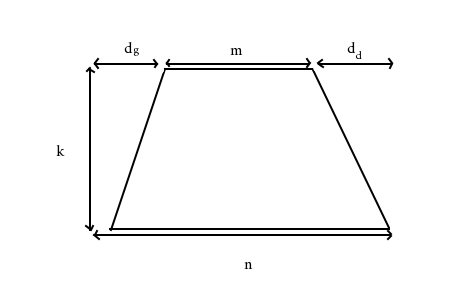
\includegraphics[height=0.4\textheight]{../img/trapeze.jpg}
			\end{center}
			\onslide<3-> \item Chaque trapèze pointe vers l'entité suivante $\rightarrow$ parcours facile du tricot
			\onslide<4-> \item Pour relier/séparer des pièces : \texttt{link} et \texttt{split}
		\end{itemize}
}

\frame{
	\frametitle{Un exemple}
	\begin{center}
	\begin{tikzpicture}[scale = 0.05]
		\tikzstyle{fleche}=[->,>=latex,line width=1mm]
		\fill[color=gray!20] (0,0) -- (60,0) -- (60,120) -- (0,120) -- cycle;
		\fill[color=white] (30,30) -- (45,60) -- (30,90) -- (15,60) -- cycle;
		\draw[thick] (0,0) -- (60,0) -- (60,120) -- (0,120) -- cycle;
		\draw[thick] (0,30) -- (60,30) ;
		\draw[thick] (0,90) -- (60,90) ;
		\draw[thick] (0,60) -- (15,60) ;
		\draw[thick] (45,60) -- (60,60) ;
		\draw[thick] (30,30) -- (45,60) -- (30,90) -- (15,60) -- cycle;

		\onslide<2->
		\draw[fleche, color=red] (30,20) -- (15,40);
		\draw[fleche, color=red] (30,20) -- (45,40);
		\draw[color=red] (30,15) node{split};
		\draw[fleche, color=blue] (8,50) -- (8,70);
		\draw[fleche, color=blue] (52,50) -- (52,70);
		\draw[color=blue] (30,60) node{next};
		\draw[fleche,color=green] (15,80) -- (30,100);
		\draw[fleche,color=green] (45,80) -- (30,100);
		\draw[color=green] (30,105) node {link};
		\draw (30,-10) node{start};
		\draw[fleche] (30,-5) -- (30,10);
		\draw (30,130) node{stop};
		\draw[fleche] (30,110) -- (30,125);
	\end{tikzpicture}
	\end{center}
}

\subsection{Conception d'un compilateur}

\frame{
	\frametitle{Le compilateur}
		\begin{itemize}
			\onslide<1-> \item Pouvoir passer d'un tricot à une liste d'instructions pour le réaliser.
			\onslide<2-> \item Mais aussi la détection d'erreurs, par exemple la présence d'un cycle dans la description du tricot.
			\onslide<3-> \item Pour ce faire, le compilateur construit un graphe de dépendances, qui indique pour chaque pièce, les pièces qu'il faut tricoter au préalable.
			\onslide<4-> \item Pour mettre en évidence les sections qui se tricotent de manière séquentielle, ce graphe utilise une représentation en blocs de base, de manière similaire aux compilateurs, afin de simplifier l'analyse et la traduction du code.
		\end{itemize}
}

\subsection{Elaboration d'une interface}

\frame{
	\frametitle{L'interface graphique}
		3 objectifs :
		\begin{itemize}
			\item Simple d'utilisation
			\item Outils d'éditions
			\item Appel au compilateur
		\end{itemize}
}

\frame{
	\begin{center}
		\Huge{Démo !}
	\end{center}
}

\section{Difficultés rencontrées \& améliorations possibles}

\subsection{Difficultés}

\frame{
	\frametitle{Difficultés rencontrées}
		\begin{itemize}
			  	\onslide<2-> \item \textcolor{red}{Première étape de conception du langage sous-estimée...} \\
				\onslide<3-> \textcolor{vert}{$\longrightarrow$ mais un langage plus complet dès le début}
				\onslide<4-> \item \textcolor{red}{Mais également la conception de l'interface (surtout le temps nécessaire)}
				\onslide<5-> \item \textcolor{red}{Mise en route difficile...} \\
				\onslide<6-> \textcolor{vert}{$\longrightarrow$ mais l'intégration des différents modules a été plus simple que prévue}
    	\end{itemize}
}

\subsection{Améliorations}

\frame{
  \frametitle{Améliorations en perspective...}
  \begin{itemize}
    \onslide<2-> \item Édition : plus de liberté dans la personnalisation
    \begin{itemize}
      \onslide<3-> \item Des points définis par l'utilisateur
    \item Pouvoir ajouter des tresses
      \begin{itemize}
      \item Définition de zones sur les trapèzes ?
      \end{itemize}
    \item Changer la taille des pièces, ...
    \end{itemize}
    \onslide<4-> \item Côté compilateur :
    \begin{itemize}
      \onslide<5-> \item gérer les coutures (à effectuer après le tricot)
    \end{itemize}
  \item Amélioration de l'interface graphique
  \end{itemize}
}

\frame{
	\begin{center}
		\Huge{Des questions ?}
	\end{center}
}

\end{document}
